\documentclass{ximera}

\newcommand{\RR}{\mathbb R}
\renewcommand{\d}{\,d}
\newcommand{\dd}[2][]{\frac{d #1}{d #2}}
\renewcommand{\l}{\ell}
\newcommand{\ddx}{\frac{d}{dx}}
\newcommand{\dfn}{\textbf}
\newcommand{\eval}[1]{\bigg[ #1 \bigg]}


\author{Jim Talamo}

\outcome{Compute the length of a parametric curve.}

\begin{document}
\begin{exercise}
Consider the curve shown below, which is traced out by $\vec{p}(t)$.

\begin{center}

    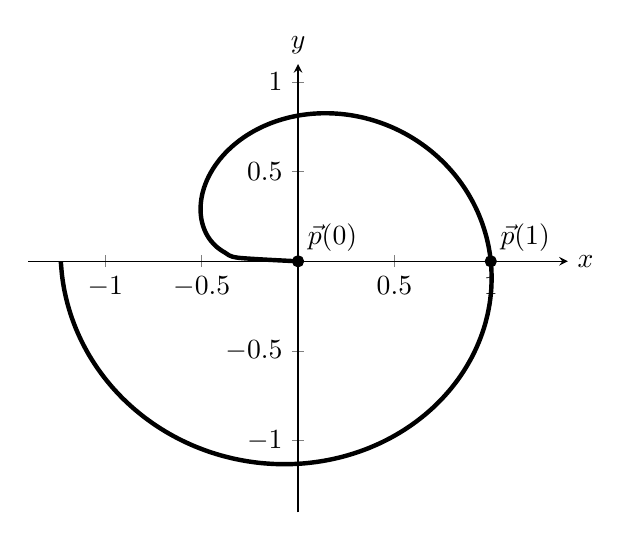
\begin{tikzpicture}
      \begin{axis}[
          xmin=-1.4, xmax=1.4, ymin =-1.4, ymax = 1.1,
          axis lines=center,  
          xlabel=$x$,  
          ylabel=$y$,  
          every axis y label/.style={at=(current axis.above origin),anchor=south},  
          every axis x label/.style={at=(current axis.right of origin),anchor=west}
        ]
        \addplot [black,ultra thick,domain=0:360,smooth,samples=100] ({-((x/180)^(.3))*cos(x)},{((x/180)^.3)*sin(x)});
        \node[above right,black] at (axis cs: 0,0) {$\vec{p}(0)$};
        \node[above right,black] at (axis cs: {-((180/180)^(.3))*cos(180)},{((180/180)^.3)*sin(180)}) {$\vec{p}(1)$};
        

        \addplot[color=black,fill=black,only marks,mark=*] coordinates{(-{((180/180)^(.3))*cos(180)},{((180/180)^.3)*sin(180)})};
        \addplot[color=black,fill=black,only marks,mark=*] coordinates{(0,0)};
        
      \end{axis}
    \end{tikzpicture}
\end{center}

If the curve does use arclength as a parameter, what must be true?
\begin{selectAll}
\choice[correct]{$\left|\vec{p}'(t)\right|$ should be $1$ for all $t$.}
\choice{$\left|\vec{p}'(t)\right|$ must be $1$ for some $t>0$, but not necessarily for all $t$.}
\choice[correct]{$\int_0^t \left|\vec{p}'(\tau)\right| \d \tau = t$ for all $t$.}
\choice{$\int_0^t \left|\vec{p}'(\tau)\right| \d \tau = t$ for some $t>0$, but not necessarily for all $t$.}
\choice{$|\vec{p}(t)| = t$ for all $t$.}
\choice{$|\vec{p}(t)| = t$ for some $t>0$, but not necessarily for all $t$.}
\end{selectAll}

Is the curve parameterized by arclength? 

\begin{multipleChoice}
\choice{Yes.}
\choice[correct]{No.}
\choice{It does, but only for some values of $t$.}
\end{multipleChoice}

\begin{feedback}[correct]
If $\vec{p}(t)$ is a parameterization of the curve that uses arclength as a parameter, then $\vec{p}(1)$ should give the $x,y$-coordinates after we have travelled $1$ unit along the curve.  From the picture, we have travelled much farther than $1$ unit, since the only way we can start at the origin, travel $1$ unit, and arrive at $(1,0)$ is to travel along the line from $(0,0)$ to $(1,0)$.
\end{feedback}

\end{exercise}
\end{document}
